\section*{Problema 3}

\textbf{Dado un conjunto de puntos ($x_i,y_i$) con $i=0,1,2,\dots,n$ con $x_i<x_j$ para $i<j$. Determine el spline de grado 1 y que pasa por los puntos ($x_i,y_i$).}

Al ser ecuaciones de lineas, entonces no se puede asegurar que $S(x)$ sea diferenciable en $[x_i,x_n]$, por lo que, se tratará a cada parámetro del spline como independiente, esto es, formar una ecuación de la recta que pase por los puntos $(x_i,x_{i+1})$. Entonces se tiene lo siguiente:

\begin{align}
    a_i & = \frac{y_{i+1}-y_{i}}{x_{i+1}-x_i} \label{eq:ai} \\
    b_i & = y_i - a_i x_i \label{eq:bi}
\end{align}

Se crearon puntos consecutivos dados por la ecuación \ref{eq:problema4x}.

\begin{equation}
    x = x_i + \frac{i(x_f-x_i)}{n-1} \qquad i=0,1,2,\dots,n \label{eq:problema4x}
\end{equation}

Donde $x_i,x_f$ es el límite inferior y superior del intervalo y n es el número de puntos que se quieren generar. Para este ejercicio se hizo uso de la ecuación \ref{eq:problema4_fx} para interpolar.

\begin{equation}
    f(x) = x^2-4x+10+2\sin ( 10x)-5 \cos (4x) \label{eq:problema4_fx}
\end{equation}

La interpolación se realizo con $n=\{10,25,50,100\}$ para el intervalo $[0,5]$. En la figura \ref{fig:problema4} se muestra la interpolación de la ecuación \ref{eq:problema4_fx}.

\begin{figure}[H]
    \centering
    \begin{subfigure}[b]{8cm}
        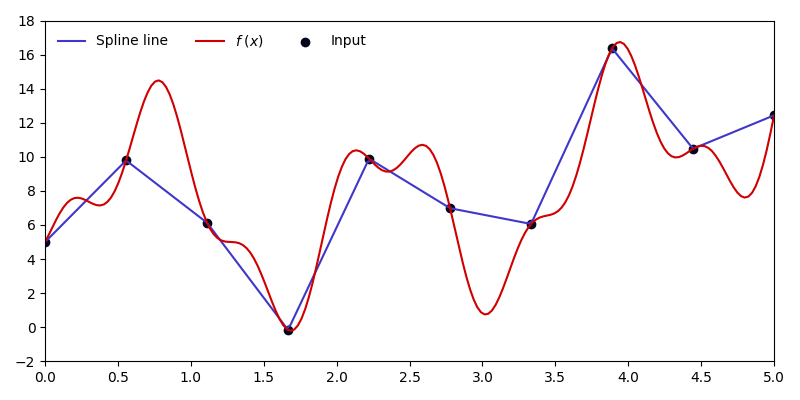
\includegraphics[width=8cm]{Graphics/problema3_10.png}
        \caption{$n=10$}
    \end{subfigure}
    \begin{subfigure}[b]{8cm}
        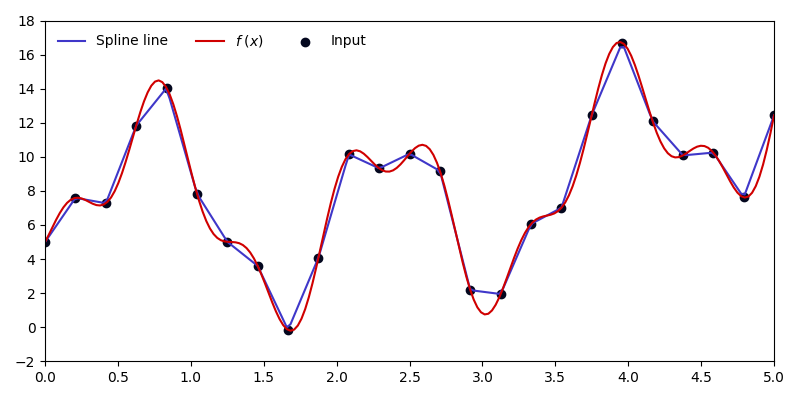
\includegraphics[width=8cm]{Graphics/problema3_25.png}
        \caption{$n=25$}
    \end{subfigure}
    \begin{subfigure}[b]{8cm}
        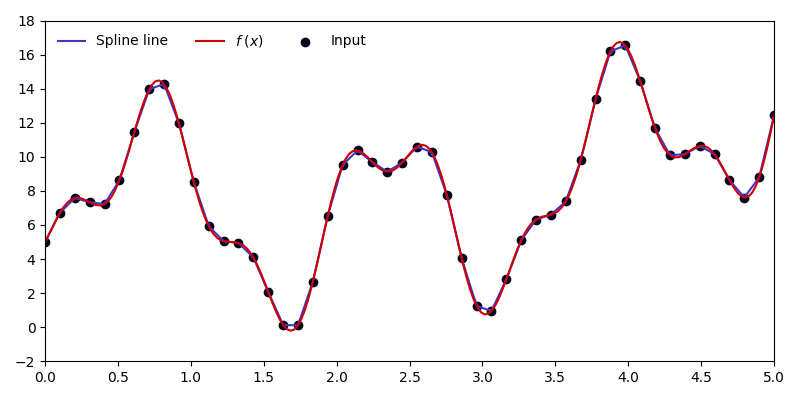
\includegraphics[width=8cm]{Graphics/problema3_50.png}
        \caption{$n=50$}
    \end{subfigure}
    \begin{subfigure}[b]{8cm}
        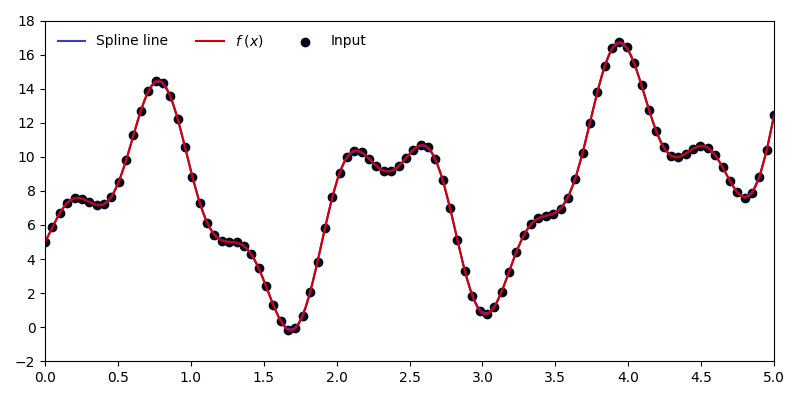
\includegraphics[width=8cm]{Graphics/problema3_100.png}
        \caption{$n=100$}
    \end{subfigure}
    \caption{Spline lineal de la ecuación \ref{eq:problema4_fx} para diferentes números de input.}
    \label{fig:problema4}
\end{figure}

Con estos resultados se obtiene que a un mayor número de inputs se obtiene una mejor interpolación para la función original de los datos.
\pagebreak